\documentclass[11pt, french]{article}
\usepackage{calc}
\usepackage{eso-pic}

\newlength{\PageFrameTopMargin}
\newlength{\PageFrameBottomMargin}
\newlength{\PageFrameLeftMargin}
\newlength{\PageFrameRightMargin}

\setlength{\PageFrameTopMargin}{1.5cm}
\setlength{\PageFrameBottomMargin}{1cm}
\setlength{\PageFrameLeftMargin}{1cm}
\setlength{\PageFrameRightMargin}{1cm}

\makeatletter

\newlength{\Page@FrameHeight}
\newlength{\Page@FrameWidth}

\AddToShipoutPicture{
  \thinlines
  \setlength{\Page@FrameHeight}{\paperheight-\PageFrameTopMargin-\PageFrameBottomMargin}
  \setlength{\Page@FrameWidth}{\paperwidth-\PageFrameLeftMargin-\PageFrameRightMargin}
  \put(\strip@pt\PageFrameLeftMargin,\strip@pt\PageFrameTopMargin){
    \framebox(\strip@pt\Page@FrameWidth, \strip@pt\Page@FrameHeight){}}}

\makeatother
%%%%%%%%%%%%%%%%%%%%%%%%%%%%%%%%%%%%%%%%%%%%%%%%%%%%%
% Importation des paquets
%%%%%%%%%%%%%%%%%%%%%%%%%%%%%%%%%%%%%%%%%%%%%%%%%%%%%
\usepackage[utf8]{inputenc}
\usepackage{helvet}
\usepackage{natbib}
\usepackage{graphicx}
\usepackage{libertine}
\usepackage{eso-pic}
\usepackage{hyperref} % allow to write hyperlink (open the url)
\usepackage{titlesec} % allow to change fontsize of the different section
\usepackage{tabularx} % allow to create tables with fixed length
\usepackage{listings} % code highlighting
\usepackage{xcolor}
\usepackage{amsmath}
\usepackage{amssymb}

\usepackage[a4paper,margin=1in]{geometry}
\definecolor{LightGray}{gray}{0.9}


%%%%%%%%%%%%%%%%%%%%%%%%%%%%%%%%%%%%%%%%%%%%%%%%%%%%%
% Definition des commandes
%%%%%%%%%%%%%%%%%%%%%%%%%%%%%%%%%%%%%%%%%%%%%%%%%%%%%
% Permet de définir une image en arrière plan
\newcommand\BackgroundPic{%
\put(0,0){%
\parbox[b][\paperheight]{\paperwidth}{%
\vfill
\centering
\includegraphics[width=\paperwidth,height=\paperheight]{background-42-ai.png}%
\vfill
}}}

% Définition de la commande pour faire un snippet de code inline
\newcommand{\inlsnippet}[1]{\colorbox{gray!10}{\mbox{\textcolor{pink}{#1}}}}

% Modification of the style of hyperlink, to be visible
\hypersetup{
    colorlinks=true,
    linkcolor=blue,
    filecolor=magenta,      
    urlcolor=cyan,
}

%%%%%%%%%%%%%%%%%%%%%%%%%%%%%%%%%%%%%%%%%%%%%%%%%%%%%%%%%%%%%%%%%%%%%%%%%%%
% Definition of black backgrounded Python code snippet
%%%%%%%%%%%%%%%%%%%%%%%%%%%%%%%%%%%%%%%%%%%%%%%%%%%%%%%%%%%%%%%%%%%%%%%%%%%
\definecolor{pink}{HTML}{ff33cc}
\definecolor{codewhite}{HTML}{ffffff}
\definecolor{codegreen}{HTML}{00e600}
\definecolor{codelemon}{HTML}{99ff99}
\definecolor{codegray}{HTML}{bfbfbf}
\definecolor{codepurple}{HTML}{9933ff}
\definecolor{codeblue}{HTML}{0099ff}
\definecolor{codered}{HTML}{ff3333}
\definecolor{bg}{HTML}{000000}

\lstdefinestyle{nightly}{
    language=Python,
    backgroundcolor=\color{bg},   
    commentstyle=\fontfamily{cmss}\color{codegreen},
    keywordstyle=\fontfamily{cmss}\color{codeblue},
    otherkeywordstyle=\fontfamily{cmss}\color{codered},            
    numberstyle=\fontfamily{cmss}\small\color{codegray},
    stringstyle=\fontfamily{cmss}\color{codepurple},
    basicstyle=\fontfamily{cmss}\small\color{codewhite},
    emph={def,is,not,in,False,True,as,and,or,from},
    emphstyle={\fontfamily{cmss}\small\color{pink}},
    emph={[2]MyClass,__init__,__repr__,__print__},
    emphstyle={[2]\fontfamily{cmss}\small\color{codered}},
    emph={[3]str,float,tuple,int,list},
    emphstyle={[3]\fontfamily{cmss}\small\color{codelemon}},
    breakatwhitespace=false,         
    breaklines=true,                 
    captionpos=b,                    
    keepspaces=true,                 
    numbers=left,                    
    numbersep=5pt,                  
    showspaces=false,                
    showstringspaces=false,
    showtabs=false,                  
    tabsize=2
}
%%%%%%%%%%%%%%%%%%%%%%%%%%%%%%%  End of definition  %%%%%%%%%%%%%%%%%%%%


%%%%%%%%%%%%%%%%%%%%%%%%%%%%%%%%%%%%%%%%%%%%%%%%%%%%%
% Titre, date, auteur
%%%%%%%%%%%%%%%%%%%%%%%%%%%%%%%%%%%%%%%%%%%%%%%%%%%%%

\author{} %\author{42-AI}
\title{Practise sheet}
%\maketitle

%%%%%%%%%%%%%%%%%%%%%%%%%%%%%%%%%%%%%%%%%%%%%%%%%%%%%
% Début du document
%%%%%%%%%%%%%%%%%%%%%%%%%%%%%%%%%%%%%%%%%%%%%%%%%%%%%
\begin{document}


%%% >>>>> Page de garde
\vspace*{2cm}
\begin{center}
    \textsc{\fontsize{40}{48} \bfseries Practise Sheet 5}\\[0.6cm]
    \textsc{\fontsize{40}{48} \bfseries Analysis}\\[0.3cm]
\end{center}
\vspace{3cm}

\begin{figure}[!h]
\center

\includegraphics[scale=0.5]{logo-42-ai.png}
\label{fig:1st_page_logo_42ai}
\end{figure}

\vspace*{2cm}
\begin{center}
    \textsc{\fontsize{32}{48} \bfseries Dérivation de fonction à une seule variable}\\[0.6cm]
\end{center}
\vspace{3cm}

\pagenumbering{gobble}
\newpage


%%% >>>>> Document body

\section*{Objectifs:}
L'objectif principal de cette série d'exercices est de vous entraîner à dériver des fonctions à une seule variable.
Lorsque vous réaliserez vos modèles, ceux-ci peuvent être basés sur des fonctions très diverses, de même que la fonction de coût qui peut être la distance quadratique moyenne ou bien une toute autre fonction.


\subsection*{Préambule:}
Dans votre cursus classique, vous étudiez la notion de de taux de variation, puis la dérivée d'une fonction en un point, suivi de la détermination de la tangente d'une fonction en un point d'abscisse $a$ et cela en long et en large.\
Ces notions sont importantes à comprendre pour saisir le sens de la dérivation, mais la notion sur laquelle nous allons nous attarder le plus est la détermination de l'expression dérivée d'une fonction.\
La dérivation d'une fonction vous sera utile pour déterminer l'expression de la dérivée de la fonction de coût, mais également pour déterminer le vecteur Jacobien et la matrice Hessienne que nous verrons plus tard à la fin de la partie sur l'algèbre.


\section*{Exercice 1:}
Cette exercice traite de la notion du taux de variation.\\
L'objectif est que vous compreniez quelle information donne le taux de variation et quelles informations le taux de variation ne donne pas.

\subsection*{Partie 1:}
Sur la figure ci-dessous est représenté la fonction $f$ d'équation:
\begin{equation*}
    f(x) = x^3-6x^2+4x+12
\end{equation*}

Calculer le  taux de variations entre les points:
\begin{itemize}
    \item $(-5, f(-5))$ et $(-3, f(-3))$,
    \item $(-3, f(-3))$ et $(-2, f(-2))$,
    \item $(-3, f(-3))$ et $(0, f(0))$,
    \item $(0, f(0))$ et $(1, f(1))$,
    \item $(0, f(0))$ et $(4, f(4))$,
    \item $(4, f(4))$ et $(7, f(7))$,
\end{itemize}

\textit{Évidemment vous devez calculer in fine les valeurs de la fonction pour les différents points mentionnés.}\\
\textbf{Petite précision}, lorsque l'on vous dit de calculer le \textbf{taux de variation entre le points $\mathbf{(a, f(a))}$ et $\mathbf{(b, f(b))}$} cela donne:
\begin{equation*}
    \tau_f(a,b) = \frac{f(b)-f(a)}{b-a}
\end{equation*}

\begin{figure}[!h]
\center
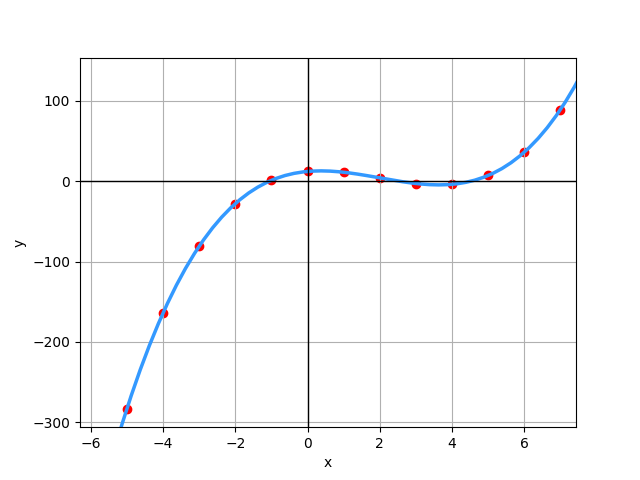
\includegraphics[scale=0.8]{assets/serie_5_exo_1_figure_1.png}
\label{fig:p_s_5_exo1-fig1}
\end{figure}

\subsubsection*{Questions:}
\begin{enumerate}
    \item Que pouvez-vous dire entre le taux de variation et l'évolution de la fonction ?
    \item Y-a-t-il un lien entre le taux de variation de la fonction entre 2 points et l'évolution de la fonction entre ceux-ci ? 
\end{enumerate}

\subsection*{Partie 2:}
\subsubsection*{Questions:}
\begin{enumerate}
    \item Calculer maintenant le taux de variation entre les points $(-2, f(-2))$ et $(6,f(6))$.
    \item Le taux de variation calculé donne-t-il l'information que la fonction est croissante, décroissante puis recroissante sur l'intervalle $[-2;6]$ ?
    \item L'information sur l'évolution obtenue par le taux de variation est de quelle nature ? (locale ?, globale ?, instantanée ?, moyennée ?)
\end{enumerate}

\subsection*{Partie 3: Coding time !}
Vous devez coder une fonction permettant de calculer le taux de variation d'une fonction.
\begin{enumerate}
    \item Dans un premier temps, la fonction recevra en paramètre 2 tuples de 2 nombres:
    \begin{lstlisting}[style=nightly]
        import sympy as sy
        
        def variation_rate(tuple_A, tuple_B):
            """
            Parameters
                tuple_A : tuple of 2 numbers corresponding to x and y
                of point A.
                tuple_B : tuple of 2 numbers corresponding to x and y
                of point B.
            Description:
                Function calculates the variation rate between A and B.
            Return:
                tau_AB: variation rate between A and B.
            """
            "Your code here."
        
        x = sy.Symbol('x')
        f = 3*x + 12
        A = (1, f.subs(x,1))
        B = (2, f.subs(x,2))
        variation_rate(A,B)
        # Output:
        3.0
    \end{lstlisting}
    \item Coder une version améliorée de la fonction \inlsnippet{variation_rate} qui prendra 3 paramètres:
    \begin{itemize}
        \item une liste ou une tuple de 2 nombres délimitant l'intervalle où l'on calcul le taux de variation,
        \item une fonction,
        \item un nombre exprimant le nombre de segment subdivisant l'intervalle pour lesquels le taux de variation est calculé.
    \end{itemize}
    \begin{lstlisting}[style=nightly]
        import sympy as sy
        
        def variation_rate(interval, f, nb_seg):
            """
            Parameters
                tuple_A : tuple of 2 numbers corresponding to inf and
                max of the interval.
                f : expression of a function.
                nb_seg: number of segments on which variation rate will
                be calculated
            Description:
                Function calculates the nb_seg variation rate of f
                on interval.
            Return:
                list containing the abcissas, values fonctions and
                variation rate:
                [x1, x2, f(x1), f(x2), (f(x2) - f(x1))/(x2 - x1)]
            """
            "Your code here."
        
        x = sy.Symbol('x')
        f = 3*x + 12
        interval =  (0, 5)
        
        variation_rate(interval,f, 5)
        # Output:
        [[0, 1, 12, 15, 3],
         [1, 2, 15, 18, 3],
         [2, 3, 18, 21, 3],
         [3, 4, 21, 24, 3],
         [4, 5, 24, 27, 3]]
    \end{lstlisting}
    \item[3] Calculer à l'aide de votre fonction, le taux de variation de f sur différents intervalles et pour des couples de points de plus en plus proche (en précisant des points plus proches dans \inlsnippet{interval} ou en augmentant \inlsnippet{nb\_seg}).
\end{enumerate}
\vspace{1cm}

\section*{Exercice 2}
\subsection*{Partie 1:}
Nous allons étudier le lien entre taux de variation et nombre dérivée en un point à l'aide de la formule de la limite:
\begin{equation*}
    f'(a) = \lim_{\delta \rightarrow 0} \frac{f(a+\delta) + f(a)}{\delta}
\end{equation*}

Pour cela, considère la fonction:
\begin{equation*}
    f(x) = 3x^3 - 6x^2 + 5
\end{equation*}

1. Calculer le taux de variation de la fonction pour les points d'abscisses $-1$, $0$ et $1$ pour $\delta$ étant égale à $1$, $0.1$, $0.01$ et $0.001$.
2. Montrer que la dérivée de la fonction f a pour expression:
\begin{equation*}
f'(x) = 9x^2 - 12x
\end{equation*}
\begin{enumerate}
    \item Calculer les valeurs de $f'(x)$ pour x égal à $-1$, $0$ et $1$.
    \item Vers quelles valeurs tendent les taux de variation de f en $-1$, $0$ et $1$ ?
\end{enumerate}

\subsection*{Partie 2:}
La notion de tangente est liée à celle de dérivée.
En effet, l'équation d'une tangente à une fonction au point d'abscisse $a$, est rattachée la dérivée au point $a$ de la fonction f (c'est-à-dire $f'(a)$):
\begin{equation*}
    f'(a)(x-a) + f(a)
\end{equation*}

\begin{enumerate}
    \item Donner les expressions des tangentes à la fonction $f$ aux points d'abscisses $-2$, $0$ et $2$\\
    \item À l'aide de la librairie \inlsnippet{matplotlib.pyplot} tracer la fonction $f$ ainsi que les tangentes aux différents points d'abscisses $-2$, $0$ et $2$.
    \item Coder une fonction permettant de déterminer l'expression de la tangente (utiliser la méthode \inlsnippet{diff} au sein de \inlsnippet{sympy}):
\end{enumerate}

\begin{lstlisting}[style=nightly]
    def tangent(f, a):
        """
        Parameters
            f : expression of a function.
            a: abscissa where the tangent is calculated.
        Description:
            Function calculates the tangent.
        Return:
            the expression of the tangent at a.
        """
    
    import sympy as sy
    x = sy.Symbol('x')
    f = 3*x**2 + 12
    tangent(f, 5)
    # Output:
    30x-63
\end{lstlisting}

À l'aide de la fonction \inlsnippet{tangent} calculer la tangente des fonctions suivantes:
\begin{align*}
   f(x) =& \frac{1}{2}x^2 + 3 \\
   g(x) =& \frac{1}{3}x^3 + \frac{1}{2}x^2 + x \\
   h(x) =& \frac{1}{4}x^4 - 3x^3 + 2x  -6 
\end{align*}

aux points de d'abscisses $-1$, $0$, $1$ et $4$.\\
Tracer sur 3 figures différentes les fonctions et leurs tangentes aux différents points.\\
Observez que les pentes des tangentes aux courbes des fonctions, aux points concernés, correspondent aux taux de variations ("instantanées") des fonctions en ces points.
\vspace{1cm}

\section*{Exercice 3}
Dans cette exercice, vous allez vous entraînez à dériver quelques fonctions.
Le but n'étant pas de faire de vous des experts de la dérivation, \inlsnippet{sympy} le fait très bien, et en une seule commande : \inlsnippet{sympy.diff}. L'objectif est donc que vous saisissiez le concept de dérivation et que vous puissiez manipuler la dérivation au cours de vos raisonnements futur sur la bonne vieille feuille de papier.

Afin de vous faciliter la vie avec la dérivation, connaître un minimum de dérivée usuelle et quelques règles de dérivation n'est pas du luxe, et c'est ce que nous allons voir.

\subsection*{Partie 1: Dérivée d'une somme de fonction}
La première règle de dérivation est que la dérivée d'une somme de fonction est égale à la somme des dérivées des fonctions.
\begin{equation*}
\frac{d}{dx}(f(x)+g(x)) = \frac{df}{dx} + \frac{dg}{dx}
\end{equation*}

\begin{itemize}
    \item Calculer les dérivées des fonctions suivantes:
\end{itemize}

\begin{align*}
\begin{matrix}
f_1(x) =& \frac{1}{2}x^2, & f_2(x) = & 3x^3,                & f_3(x) = & 2\sqrt{x},\\
f_4(x) =& 3x^3 + 2x,      & f_5(x) = & 3x^3+ 5x^2 + 6x + 1, & f_6(x) = & 2\sqrt{x}+ \frac{1}{16}x^4 + \frac{1}{x},\\
f_7(x) =& x^10 + \frac{1}{x^5} - 5\sqrt{x}, & f_8(x) = & \sum_{i=1}^{N}ix^i, & f_9(x) = & \sum_{i=1}^{N}\frac{i}{x^i},
\end{matrix}
\end{align*}

\subsection*{Partie 2: Dérivée d'un produit de fonctions}
La seconde règle de dérivation concerne la dérivée d'un produit de fonctions. Celle-ci est définie telle que:
\begin{equation*}
    \frac{d}{dx}(f(x)\times g(x)) = \frac{df}{dx}\times g(x) + f(x) \times \frac{dg}{dx}
\end{equation*}

\begin{itemize}
    \item Calculer les dérivées des fonctions suivantes:
\end{itemize}

\noindent\rule{\textwidth}{1pt}
\subsubsection*{Note:}
\begin{equation*}
    \frac{d}{dx} \left( cos(x)\right) = -sin(x) \quad \quad \frac{d}{dx} \left( sin(x)\right) = cos(x)
\end{equation*}
\noindent\rule{\textwidth}{1pt}

\begin{equation*}
\begin{matrix}
f_1(x) = & \left(\frac{1}{2}x^2 \times \sqrt{x}\right) & f_2(x) = 3x^3\times cos(x) & f_3(x) = 2\sqrt{x}\times sin(x)\\
f_4(x) = & cos(x)\times sin(x) & f_5(x) = x^4\times cos(x)\times \sqrt{x} & f_6(x) = ln(x)\times e^x\\
\end{matrix}
\end{equation*}

\subsection*{Partie 3: Dérivée d'une composition de fonctions}
La troisième règle de dérivation concerne la composition de fonctions. Celle-ci est définie telle que:
\begin{equation*}
\frac{d}{dx}(f(u(x)) = u'(x)\times f'(u(x)) 
\end{equation*}
Calculer les dérivées des fonctions suivantes:

\begin{equation*}
\begin{matrix}
f_1(x) = &  3\left(x^2 + 1\right)^2 & f_2(x) = & 3\left(x^5 + 1\right)^3 & f_3(x) = &\sqrt{\frac{1}{2}x^2}\\
f_4(x) = & (2\sqrt{x}- 3)^4 & f_5(x) = & \frac{2}{x^2-5} & f_6(x) = & e^{3x^3 -1}\\
\end{matrix}
\end{equation*}


%\begin{lstlisting}[style=nightly]
%import numpy as np
%def test_function:
 %   """
 %   Description..
 %   """
 %   for i in range(0,5):
 %       list()
 %       int()
 %       return
 %   
 %   # comment
 %   x = 2
 %   test_function()
%\end{lstlisting}

\end{document}
%%%%%%%%%%%%%%%%%%%%%%%%%%%%%%%%%%%%%%%%%%%%%%%%%%%%%